\chapter{Introduction}\label{chapter:intro}

\epigraph{“Don’t be scared. All of this is new to you, and new can be scary. Now we all want answers. Stick with me — you might get some.”}{\textit{The 13th Doctor} - Doctor Who}
%\epigraph{I'm the Doctor; I'm worse than everyone's aunt. And that is not how I'm introducing myself.}{\textit{The 11th Doctor} - Doctor Who}
% \epigraph{Sometimes a scream is better than a thesis.}{\textit{Manfred Eigen}}

Static program analysis is the cornerstone of several modern programming
facilities and tools for program development and aided program understanding.
Nowadays, it is an umbrella term for many different methodologies (...) all
with the ultimate goal of inferring a program's properties, without the need of
an actual execution. It is routinely employed in many different contexts:
compilers, bug detectors, verifiers, security analyzers, IDEs, and a myriad
other tools.

The main intention of any \emph{static} program analysis algorithm is to reason
about the set of all feasible behaviors (under some abstraction of behaviors)
that a given program might exhibit under all possible executions. For example,
could this method throw a runtime exception? or is that type cast possible to
fail under some program input? etc.

Pointer analysis (also known as \emph{points-to analysis}) is a fundamental
subdomain of static program analysis that consists of computing some
\emph{abstract memory model} for a given program. The essence of such an
analysis is to compute a set of possible objects that a program variable or
expression may point to during program execution. A straightforward endeavor at
first, it quickly gets too complicated in practice due to all of the intricate
details one has to take into account and the multitude of different features
that mutually depend on each other. Although a challenging task, smart
implementations of pointer analysis can bear many benefits to client analyses
that will subsequently consume the results to reason about specialized
behaviors (e.g., security vulnerabilities or potential optimization
opportunities).

A closely related analysis, sometimes wrongfully confused with pointer
analysis, is \emph{alias analysis} in which one computes sets of program
expressions that may alias (i.e., point to common objects) with each other.
Pointer analysis could---although it is not the only possible alternative---be
used to implement an alias analysis algorithm, and vice versa.

At the same time, programming languages are ever evolving, ever becoming
higher-level and more complex. Many abstraction levels are added throughout the
years with the aim of making the very task of programming easier for developers
allowing them to express more with less effort (e.g., in terms of lines of
code). Frequently, new features come with complicated semantics regarding their
possible implementations and usually they interact in intricate ways with
pre-existing ones.

Additionally, modern software paradigms have evolved as well. Complex design
patterns have become the norm for experienced developers, immense libraries and
frameworks are accepted as a prerequisite for any non-trivial software, and
over-involved build tools often make even the task of understanding all of the
program's dependencies a challenge.

It comes as no surprise that any kind of static analysis has struggled to keep
up with this ever-increasing complexity both in programming languages and
software. Even the seemingly simple task of computing a program's call-graph
(i.e., which methods are called at every invocation site) requires
sophisticated analysis for achieving acceptable precision. Thus, the main
emphasis of pointer analysis algorithms is on combining fairly precise modeling
of pointer behavior and memory abstractions with scalability.

\paragraph*{Thesis.}
\begin{displayquote}
It is possible to implement \emph{highly sophisticated} and \emph{precise}
	static pointer analysis algorithms without forgoing \emph{scalability}.
	Furthermore, precision and the accompanied \emph{confidence in results} is
	a spectrum and can be tweaked differently for different parts of the
	program.
\end{displayquote}

\paragraph*{Thesis.}
\begin{displayquote}
It is possible to implement \emph{highly sophisticated} and \emph{precise}
	static pointer analysis algorithms without forgoing \emph{scalability}.
	Furthermore, precision and the accompanied \emph{confidence in results} is not a global property of a given algorithm, but can be tweaked differently for different parts of the
	program.
\end{displayquote}

We provide a number of techniques for implementing scalable static pointer and
alias analyses in the setting of Java programs by configuring the analysis
strategy differently for different code parts. Additionally, we present a
couple of defensive algorithms for reporting high-confidence results even in
the presence of hostile or unknown program points.


\section{Background}

There are a few important design choices that can affect drastically the
properties a static program analysis algorithm will enjoy and the reasoning
that is required to achieve such goals.


\subsection{The \doop{} Framework}

Most of the following work and algorithms have been expressed in the \doop{}
framework \cite{oopsla:2009:Bravenboer}. \doop{} is written in the \emph{declarative} language Datalog, and
although Datalog has been used for points-to analyses in the past, \doop{} was
the first implementation to express full end-to-end context-sensitive analyses
for Java,\footnote{More specifically, the soon-to-be presented algorithms
operate on Java Bytecode---the lower-level intermediate representation used in
the Java Virtual Machine---and thus they could, in theory, be applied to any
programming language that targets the Java VM.} declaratively. This includes
handling key analysis elements such as call-graph construction as well as logic
dealing with various semantic complexities of the Java language such as native
code, reflection and exceptions. Nowadays, \doop{} offers a wide array of
intricate analyses displaying a variety of properties.


\subsection{A Datalog Primer}
\label{sec:intro:datalog}

The declarative power of \doop{} stems from the expressiveness of Datalog.
Datalog has been described in the past, at a higher level, either as Prolog
without function symbols or as SQL with support of recursion. Programs written
in Datalog are essentially logic specifications that, as a side-effect, are
also executable. One simply models the semantics for each language feature of
interest along with any reasoning rules of the desired analysis, and the
underlying engine is responsible for combining the logic specification with
input facts and, after applying a specialized computation, inferring anything
that follows given the rules and the respective input.

The aforementioned specialized computation is known as a \emph{fixed-point}
computation. All valid Datalog rules are monotonic, i.e., can only reason about
the inference of additional facts, and this is exploited by the underlying
engine in order to efficiently compute new facts in a repeating fashion until
knowledge from previous steps cannot be applied to infer anything new in the
current step. Datalog programs are contained in the \texttt{PTime} complexity
class, i.e., they can be computed in polynomial time, and vice versa, any
polynomial algorithm can be implemented as a Datalog program. Additionally,
because of the monotonic nature of rules, termination is always
guaranteed.\footnote{We will later relax these constraints by adding language
extensions that will push Datalog programs over the \texttt{PTime} class and
might invalidate the termination guarantees offered by the language. We will do
so in a principled way, allowing for greater flexibility on the algorithms that
we can express.}

A Datalog program is mainly a collection of rules with each rule contributing
to a common knowledge base. Each rule has two parts (separated by ``\dl{:-}'');
the \emph{rule-body}, on the right, that describes what conditions need to hold
in order to infer something new, and the \emph{rule-head}, on the left, that
describes what new knowledge is inferred each time. Both parts are collections
of \emph{relations} that are conceptually similar to database tables. Relations
can be connected to each other either via commas (``\dl{,}''), denoting a
logical \texttt{AND} connection similar to a database join, or via semicolons
(``\dl{;}''), denoting a logical \texttt{OR} connection.

A classic example is given below. \relname{Parent} represents the obvious
parent relationship between individuals abstracted by the two arguments,
whereas \relname{Ancestor} represents an ancestry relationship of any depth. 

\rel{Ancestor}{x, y} \dl{:-} \rel{Parent}{x, y}\dl{.}

\rel{Ancestor}{x, y} \dl{:-} \rel{Parent}{x, z}\dl{,} \rel{Ancestor}{z, y}\dl{.}

The first rule simply states that any parent relationship is also an ancestry
one. The second rule is where recursion, the true power of Datalog, shines
through. It states that whenever some \args{x} is the parent of some \args{z},
and it is already known that \args{z} is an ancestor of some \args{y}, then it
is also valid to infer that \args{x} is transitively an ancestor of \args{y}.
This second rule is where the fixed-point computation comes into play.
Depending on the input facts, the underlying engine might need to apply the
rule multiply times, each time inferring new facts that will in turn be used as
the base for further inference.


\subsection{Context Sensitivity}

Throughout the years, pointer analysis has evolved and has been the focus of
intense research. It is widely accepted to be among the most standardized and
well-understood inter-procedural (i.e., reasoning about a property taking into
account the flow of code across different program functions) analyses.

The emphasis of points-to analysis algorithms is on combining fairly precise
modeling of pointer behavior with scalability. The challenge is to pick
judicious approximations that will allow satisfactory precision at a reasonable
cost. Furthermore, although increasing precision often leads to higher
asymptotic complexity, this worst-case behavior is rarely encountered in actual
practice. Instead, techniques that are effective at maintaining good precision
often also exhibit better average-case performance, since smaller points-to
sets lead to less work.

A widely used concept that emerged as a powerful tool for tuning precision
while still achieving scalable analyses, is that of \emph{context-sensitivity}.
It consists of qualifying interesting components of an analysis, such as
program expressions, object abstractions or method invocations, with additional
\emph{context} information. The core idea being that the analysis will collapse
information (e.g., ``what objects this method argument may point to'') for
executions that result in the same context, while keep separate information for
different contexts. In essence, qualifying components with additional context
is as if each such component is replaced with multiple versions (one for each
different associated context value) and the analysis can reason individually
for each version. This approach tries to counter the loss of precision that
naturally arises in any static analysis, from conflating information of
different dynamic program paths.

Two main flavors of context sensitivity have been explored in past literature:
\begin{inparaenum}[(1)]
\item \emph{call-site sensitivity} (also known as \emph{$k$CFA}) \cite{col:1981:Sharir,thesis:Shivers} 
in which call-sites are used to qualify variables and other analysis components, essentially re-analyzing a method for different call-sites that target that method, and
\item \emph{object-sensitivity} \cite{issta:2002:Milanova,article:2005:Milanova,popl:2011:Smaragdakis} in which receiver objects of a call are used
	instead, in a similar manner.
\end{inparaenum}
Another kind of context sensitivity, known as \emph{type-sensitivity}, has also
been explored as an approximation of object sensitivity with the aim of
preserving high precision at substantially reduced cost. In type sensitivity,
upper bounds on the dynamic types of the receiver objects are employed as
context elements.

A context-sensitive analysis has a second axis of parameterization besides
context flavor---that of (max) context depth. Consequently, a common way to
describe an analysis is using the following naming scheme:
$X$-FLAVOR-sensitive+$Y$-heap, e.g., as in 3-call-site-sensitive+2-heap. Here
FLAVOR denotes the kind of context information being employed, and, $X$ and
$Y$ denote the context depth limits being used at invocation sites and at
object allocations respectively. In the previous example the analysis is
keeping track of the 3 most recent call-sites that led to the current
method call, in order to annotate local variables. Similarly, the analysis is
using the 2 most recent call-sites that led to the allocation site of an
object to annotate the newly allocated object.


\subsection{Intraprocedural vs. Interprocedural Analyses}

Different kinds of static program analysis may define differently which program
parts are of interest. An \emph{intraprocedural} analysis makes its reasoning
using only the local information that is available in each program function.
Multiple analyses commonly found in a classical compiler, such as
\emph{type-checking} or the computation of \emph{live-ranges} for program
variables are well-known examples of intraprocedural static program analyses.
On the contrary, an \emph{interprocedural} analysis is one whose reasoning
transcends function boundaries, taking into account how different functions
interact with each other. An analysis reasoning about \emph{thrown
exception}---that flow out of a function---is one such example.

Furthermore, a related categorization is that of a \emph{whole-program}
analysis in contrast to a \emph{modular} one. A whole-program analysis examines
every part of the program, including any external dependencies that the code
may have, and reasons about the effects each part has on the rest of the
program. In the setting of Java, for example, a whole-program analysis not only
reasons about the application code but additionally about any third-party
library used by the program (e.g., from external Java Archives---JARs) and also
about code run by the Java Runtime Environment---i.e, library code provided by
the language itself. On the other hand, a modular analysis only focuses on
specific parts of the program and ignores the effects of the rest (e.g., an
analysis focusing on certain Java packages).

A modular analysis usually may afford to implement more complex, more expensive
reasoning than a whole-program one, since it only focuses on a very localized
part of the program. On the contrary, a whole-program analysis has to
constantly balance the complexity of its logic,  any potential precision gains
but also any scalability penalties. The rest of this dissertation will only
focus on a few interesting whole-program analyses.


\subsection{Flow-Sensitivity} \label{flowSensitivity}

Although counter-intuitive at first, it is not unusual for a static program
analysis to be flow-\emph{insensitive}. A flow-sensitive analysis examines a
method's instructions while taking into account the order they appear in the
source code.  On the contrary, a flow-insensitive analysis examines a method's
instructions as if they were in a set, without any particular order (i.e., any
instruction could happen before any other), and as if they may repeat any
number of times.  The latter approach leads to analyses that overapproximate
the semantics of the actual code---thus potentially suffering in
precision---but it is a common tradeoff when aiming to improve the performance
of an analysis.

The penalties on performance for a flow-sensitive analysis mainly stem from the
need to keep track of what holds at \emph{every single} program point.
Potentially, this could mean that information that remains unchanged will be
duplicated on a multitude of instructions. On the contrary, a flow-insensitive
analysis will collapse information along all instructions of a method.

{
\setlength\intextsep{-10pt}
\begin{wrapfigure}{ht}{.12\textwidth}
\centering
\begin{javacode}
x = 1;
y = x;
x = 2;
\end{javacode}
\end{wrapfigure}

For the example on the side, a flow-sensitive analysis reasoning about the
values of primitive expressions might report that:
after line 1: ``$x$ has the value 1'',
after line 2: ``$x$ has the value 1'' and ``$y$ has the value 1'', and
after line 3: ``$x$ has the value 2'' and ``$y$ has the value 1''.

A flow-insensitive analysis might instead report that:
``$x$ has either the value 1 or 2'' and ``$y$ has either the value 1 or 2'',
because instructions are examined as if happening in any order.
}


\subsection{Static Single Assignment Form}

In compiler design, \emph{static single assignment form} (also known as SSA) is
a kind of code transformation in which every local variable is assigned only
once. Existing local variables in the original source code are split into
\emph{versions} (e.g., variable $x$ might be split into $x_1$ and $x_2$) with
each version being assigned only once. At program points where the value of the
original variable is read and there are multiple valid versions, as in the
point where the branches of an \emph{if-else} statement merge, a
\emph{phi-node} statement is used. This special statement bears the semantics
of somehow ``choosing'' a specific variable version to read.

\begin{figure}[h]
\begin{subfigure}{.45\textwidth}
    \begin{javacode}
    if (...) x = 10;
    else x = 20;
    y = x;
    \end{javacode}
    \caption{Original source code}
\end{subfigure}%
\hfill
\begin{subfigure}{.45\textwidth}
    \begin{javacode}
    if (...) x_1 = 10;
    else x_2 = 20;
    y = phi(x_1, x_2);
    \end{javacode}
    \caption{The equivalent SSA form}
\end{subfigure}
\caption{Example code before and after an SSA transformation}
\end{figure}

In the context of static program analysis, SSA is often used to approximate the
benefits of a flow-sensitive analysis, particularly pertaining to the handling
of local variables. This is not the case for other, more complicated language
features such as heap accesses and method invocations, but SSA provides an easy
way to pick the low-hanging fruit.

\setlength\intextsep{15pt}
\begin{wrapfigure}{ht}{.12\textwidth}
    \centering
\begin{javacodeNoLines}
x_1 = 1;
y = x_1;
x_2 = 2;
\end{javacodeNoLines}
\end{wrapfigure}

The flow-\emph{insensitive} analysis of \ref{flowSensitivity} will report quite
different results when analyzing the SSA-form analogue of the example code
(given on the side): ``$x_1$ has the value 1'', ``$y$ has the value 1'', and
``$x_2$ has the value 2''. The analysis is still examining instructions without
taking order into account, and is unable to answer questions such as ``what is
the value of variable $x$ at the end of the method'' (whether the value of
$x_1$ or $x_2$ is the final one), but nevertheless it has managed to reclaim
some of the precision that was previously lost---i.e., regarding the value of
variable $y$.


\subsection{May vs. Must Analyses}

Given an abstraction of behaviors (e.g., thrown exceptions) one can define two
interesting sets regarding the potential behaviors that a given program will
exhibit. Set $Any(P)$ is defined as containing all possible behaviors that a
program $P$ \emph{will} exhibit in \emph{some} program execution (e.g., method
$m1$ will throw exception $e1$ in one execution and exception $e2$ in another).
Respectively, set $All(P)$ is defined as containing behaviors that will appear
in \emph{every} program execution (e.g., method $m2$ will always throw
exception $e3$ during any execution). %I.e.,
\[
Any(P) := \bigcup_{e \in Executions} Behaviors(P, e)
\quad \textrm{and} \quad
All(P) := \bigcap_{e \in Executions} Behaviors(P, e)
\]

Both sets are a mathematical ideal, an answer only an oracle could provide.
But, for any realistic analysis such an endeavor is an undecidable problem.
Thus, a practical static program analysis will aim to compute an approximation
of one of the two sets. Under that definition, analyses are split mainly into
two groups depending on the kind of approximation they try to achieve. On one
hand, a \emph{may}-analysis is one that aims to \emph{over}-approximate
$Any(P)$. On the other hand, a \emph{must}-analysis is one that aims to
\emph{under}-approximate $All(P)$. %I.e.,
\[
May(P) \supseteq Any(P) \quad \textrm{and} \quad Must(P) \subseteq All(P)
\]

For the rest of this dissertation, unless otherwise noted, all described analyses
aim to compute $May(P)$, i.e., they are may analyses. This also reflects the fact
tha may analyses comprise the norm in related literature.


\subsection{Soundness \& Completeness}

The term \emph{soundness}, and its converse \emph{completeness}, originate from
formal mathematical logic where they are used in order to evaluate a \emph{proof}
system under a given \emph{model}. The model is some kind of mathematical
structure, such as sets over some domain of interest and the proof system is a
set of rules with which \emph{properties} regarding the model are proven. A
system is sound if and only if statements it can prove are indeed true in the
model (concisely given as ``claim implies truth''). A system is complete if and
only if what is true in the model can also be proven by the system (concisely
given as ``truth implies claim'').

In the context of static program analysis, the most relevant and widely used
term is that of soundness. In this setting, the analysis is making claims
regarding potential program behaviors under any program execution and the
validity of those claims constitutes whether the analysis is sound or not. More
specifically, a may-analysis is sound whenever what it claims is actually
true---i.e., the computed behaviors are an overapproximation of $Any(P)$.
Respectively, a must-analysis is sound whenever the computed behaviors are an
underapproximation of $All(P)$. A trivially sound-may analysis could simply
infer top ($\top$), i.e., every possible behavior. A trivially sound-must
analysis could simply infer the empty set ($\emptyset$), i.e., no behavior at
all.

Contrary to the prevalent use of soundness for evaluating static program
analysis algorithms, completeness is scarcely referenced---if ever. One can
easily find ``proofs of soundness'' on many publications but not the analogous
``proofs of completeness''. This is mainly because of the way analyses (may- or
must-) are defined as aiming to compute an \emph{approximation} of potential
behaviors. For example, what would the meaning of a complete may-analysis be?
Such an analysis has to abide by the definition of ``truth implies claim''. In
this case ``truth'' is any overapproximation of $Any(P)$. Consequencently, a
``complete'' may-analysis would need to compute all possible overapproximations
of $Any(P)$, and thus, the term is less relevant in the domain of static
program analysis.

Relatedly to soundness, there are two closely related terms characterizing the
validity of each claim made by the analysis. If the analysis incorrectly claims
that some behavior is among the potential program behaviors, then this
constitutes a \emph{false-positive}. E.g., if the analysis claims that method
$m1$ might throw an exception $e1$, but there is no program execution under
which this will actually occur. Similarly, if an analysis claims that some
behavior will never happen but in reality there exists a program execution
where such a behavior takes place, then this constitutes a
\emph{false-negative}. E.g., if the analysis claims that method $m2$ will never
throw an exception, but it actually does. By consequence of previous
definitions, a sound may analysis will make no false-negative claims, and a
sound must analysis will make no false-positive ones.

It is noteworthy that every static program analysis is also making negative
claims, in addition to positive ones, even if only implicitly. This is due to
an analysis not making some claim actually implicitly claiming its negation.
For example, if a may-analysis for thrown exceptions reports that method $m1$
might throw either exception $e1$ or exception $e2$, then it also implicitly
reports that the same method will never throw any other exception---given that
the analysis aims to compute an overapproximation of possible behaviors.


\subsection{Precision \& Recall}

Both a may- and a must-analysis operate under the premise of computing an
approximation of reality and thus there will always be claims that are either
extraneous or missing. Of course, any analysis should do its best to get as
close to the truth, even if the actual set of behaviors will always be out of
grasp. This calls for some \emph{quantitative} way to measure an analysis's
quality. Two such metrics have been proposed. \emph{Precision} indicates how
many of the analysis claims are actually part of the truth, whereas
\emph{recall} indicates how many of the actual true claims are also reported by
the analysis. For a formal definition supposing that:
\begin{itemize}
    \item $X$ is the number of true (actually happening) interesting behaviors
    \item $T \leq X$ is the number of correct claims made by the analysis (the \emph{true-positives})
    \item $F$ is the number of incorrect claims made by the analysis (the \emph{true-negatives})
\end{itemize}
then
\[
Precision(P) = \frac{T}{T + F}
\quad \textrm{and} \quad
Recall(P) = \frac{T}{X}
\]

A value of 1 is a perfect score, and a value of 0 is the worst one. A sound-may
analysis will have perfect recall, since it at least claims any behavior that
is actually true. A sound-must analysis will have perfect precision, since it
makes no incorrect claims (it does not report any behavior that cannot actually
occur).

Highly useful as they are, both measures have a major, unavoidable shortcoming.
It is rarely the case that
there is actual knowledge of the ground-truth. Somewhat a chicken-and-egg
problem, having an automatic way to retrieve the ground-truth for arbitrary
programs is both what a static analysis aims to achieve at its core and also
what is needed to evaluate its claims. Usually, one has to resort to observing
a limited amount of actual executions for a given program and---making the
assumption that the observations are a good enough representative---interpolate
to all possible program executions.

Furthermore, this approach makes both measures \emph{empirical}, in the sense that they measure an
analysis's performance in regards to a \emph{specific} given program. They bear no
information in regards to the analysis behavior at a theoretical level and cannot be
generalized to other programs. An analysis could be perfect for one program and
terrible for another. This could be tackled to some extent with the use of well-established \emph{benchmarking suites} during the testing phase, that aim to cover
common and interesting code patterns and program behaviors.


\subsection{Soundiness}

Although soundness seems like an essential property for any static program
analysis algorithm to have, and is quite prevalent in academic literature,
Livshits et al [...] make a strong claim that there is no practical sound
\emph{whole-program} may-analysis. Most of the time, this is a conscious
compromise on how to handle certain language features and not due to lack of
understanding. If one would attempt to soundly model such features in the
context of a may-analysis, i.e., overapproximate their effects, this would most
probably result in an analysis that is so unscalable or imprecise that is
practically \emph{useless}.

At the same time, many academic publications make claims of soundness and may
even provide some kind of ``proof of soundness'' but this is mostly in regards
to a \emph{subset} of language features---the analysis might be totally unsound
in handling all the rest. Thus, a need arises for a way to differentiate
between an analysis that tries its best to be sound and only gives up in a
well-defined language subset, and one that is simply unsound.

The term \emph{soundiness}, specific to the context of static program analysis,
was coined by [..] for such a purpose. A \emph{soundy} analysis handles most
classical, core language features in a sound manner (i.e., overapproximates)
and may only fail to do so (i.e., underapproximates) in a small well-accepted
subset of highly \emph{dynamic features}, specific to each language. Such
features include uses of \emph{reflection} or \emph{native code} in Java,
\emph{eval} in Javascript, and \emph{pointer arithmetic} in C/C++.

\subsection{A Static Program Analysis Mind Map}

\begin{figure}[htb!]
\begin{subfigure}{.47\textwidth}
    
\includegraphics[scale=.45]{assets/intro/venn-soundness-a.pdf}
    \caption{Behavior sets of actual program executions}
    \label{fig:intro:soundness-a}
\end{subfigure}
\hfill
\begin{subfigure}{.47\textwidth}
    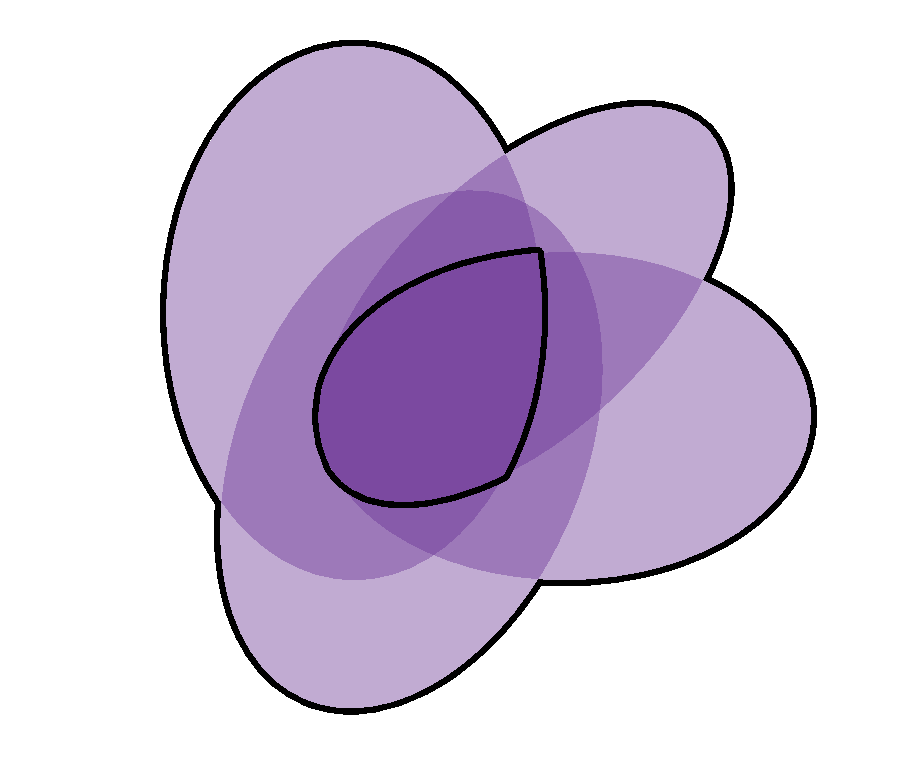
\includegraphics[scale=.45]{assets/intro/venn-soundness-b.pdf}
    \caption{Mathematical ideals $Any(P)$ (union) and $All(P)$ (intersection)}
    \label{fig:intro:soundness-b}
\end{subfigure}
\begin{subfigure}{.47\textwidth}
    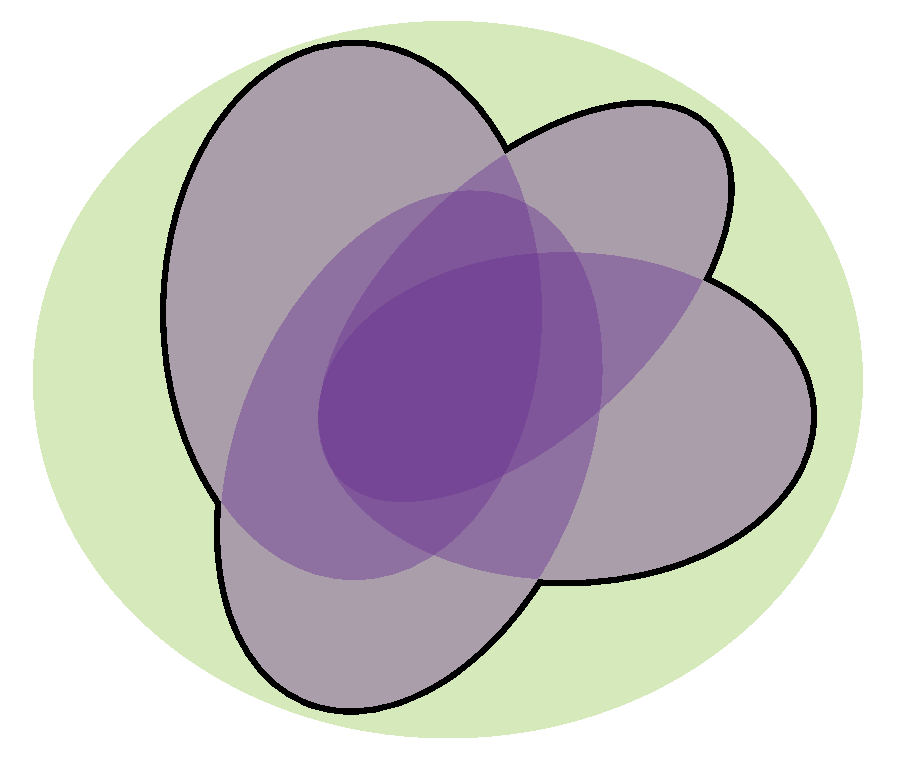
\includegraphics[scale=.45]{assets/intro/venn-soundness-c.pdf}
    \caption{Any sound-may analysis (green) in relation to $Any(P)$}
    \label{fig:intro:soundness-c}
\end{subfigure}
\hfill
\begin{subfigure}{.47\textwidth}
    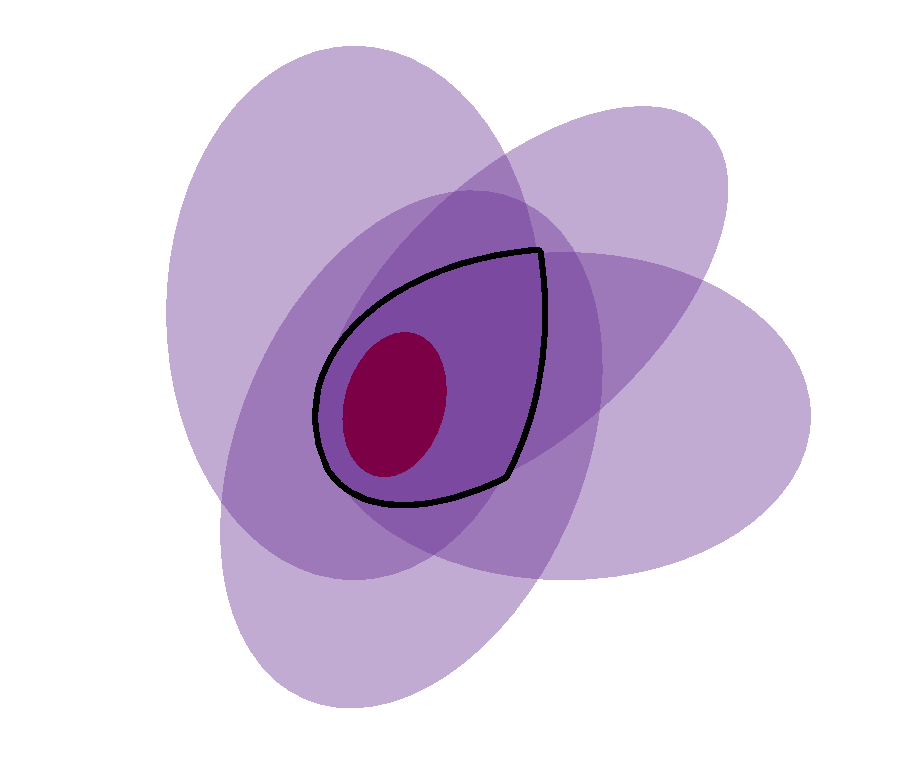
\includegraphics[scale=.45]{assets/intro/venn-soundness-d.pdf}
    \caption{Any sound-must analysis (red) in relation to $All(P)$}
    \label{fig:intro:soundness-d}
\end{subfigure}
\begin{subfigure}{.47\textwidth}
    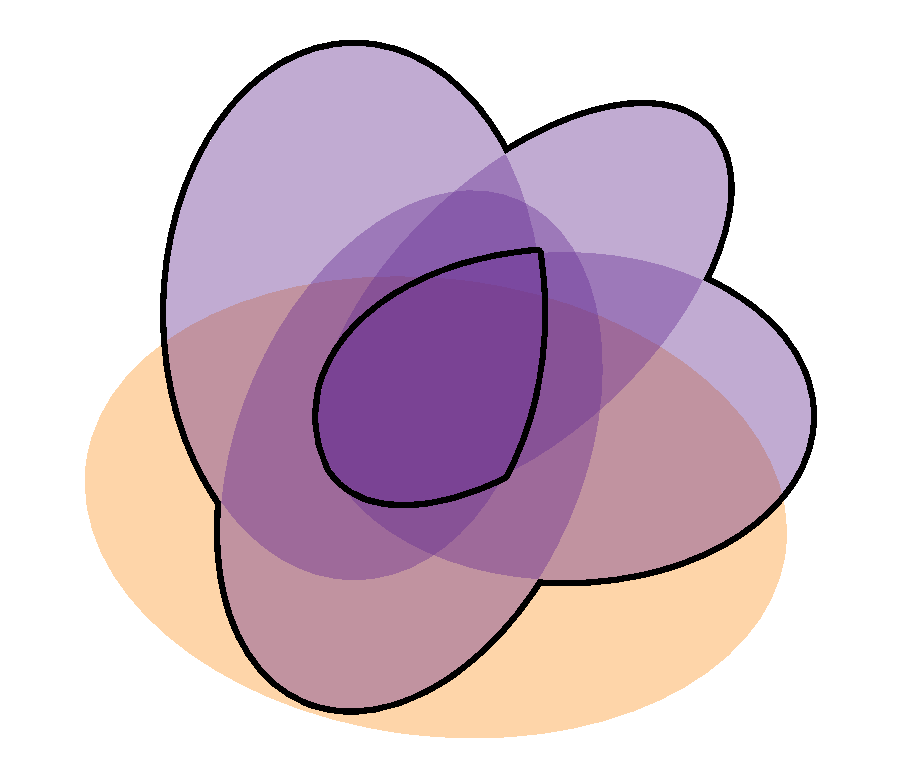
\includegraphics[scale=.45]{assets/intro/venn-soundness-e.pdf}
    \caption{Any unsound analysis (orange) in relation to both ideals}
    \label{fig:intro:soundness-e}
\end{subfigure}
\hfill
\begin{subfigure}{.47\textwidth}
    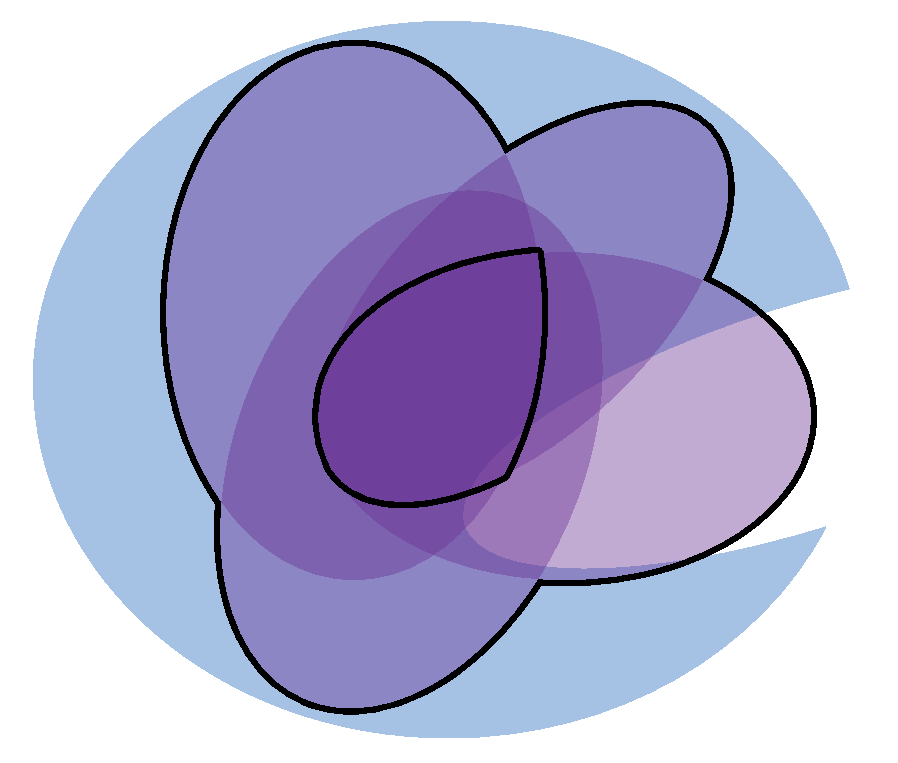
\includegraphics[scale=.45]{assets/intro/venn-soundness-f.pdf}
    \caption{Any \emph{soundy} analysis (blue) in relation to both ideals}
    \label{fig:intro:soundness-f}
\end{subfigure}
\caption{Venn diagrams visualizing the relations of different static program analysis flavors to each other and to real behaviors}
\label{fig:intro:soundness}
\end{figure}

Figure \ref{fig:intro:soundness} attempts to shed some light on how different kinds
of static program analysis relate to each other and to the mathematical ideals.
Each set in figure \ref{fig:intro:soundness-a} represents all behaviors exhibited
under a single actual program execution. Any static program analysis will
collapse different executions into a single set and will make claims about the
given program in general. In figure \ref{fig:intro:soundness-b}, the ideal $Any(P)$
is represented by the union of all sets and that of $Any(P)$ by the
intersection, respectively. Any sound-may analysis will result in a superset of
$Any(P)$ (figure \ref{fig:intro:soundness-c}), whereas any sound-must analysis will
result in a subset of $All(P)$ (figure \ref{fig:intro:soundness-d}). Finally, any
unsound analysis (figure \ref{fig:intro:soundness-e}) will result in a set with no
apparent properties; not entirely covering its appropriate mathematical ideal
but also including unrelated elements. More specifically though, as illustrated
in figure \ref{fig:intro:soundness-f}, a soundy analysis will result in a set that
starts as a superset of $Any(P)$ but misses some hard (i.e., costly) to
overapproximate behaviors in well-known cases.


\section{Scientific Contributions}

In this section, we will briefly explain the main scientific contributions of
this dissertation. As already mentioned, the exploration happens in the context
of analyzing Java---mainly by use of the \doop{} framework---although it is not
far-fetched to generalize results to other languages that offer similar
features and follow similar paradigms.

Ever since the introduction of object-sensitivity by Milanova et al. [..],
there has been increasing evidence that it is the superior context choice for
programs expressed in object-oriented languages, yielding a high precision to
cost ratio. Such has been its success that in practice it has almost superseded
the use of more traditional call-site sensitive analyses in object-oriented
languages. Nevertheless, a call-site sensitive analysis is not always inferior
as there are language features and code patterns that may partially favor this
kind of context abstraction.

Consequently, one might consider an approach where both context flavors
are---naively---combined in every program point with the goal of increasing the
precision of the end result. Truly, such a combination would bear some
precision benefits but in most cases it would be accompanied by an infeasibly
high cost.

\paragraphhead{First contribution.} Our first scientific contribution is a step towards a more sophisticated
handling aiming to achieve a beneficial combination of both context flavors. We
propose a \emph{hybrid} context flavor for defining a family of analyses where
classical contexts are mixed and combined only in those program points where it
is profitable for the analysis. The resulting selective combination of both
context kinds vastly outperforms not only analyses following the naive
non-selective combination approach, but also their ``normal'' object-sensitive
counterparts. This result holds for a large array of analyses (e.g.,
1-object-sensitive, 2-object-sensitive with a context-sensitive heap, etc.)
establishing a new set of performance/precision sweet spots.

\paragraphhead{Second contribution.} The second scientific contribution tries to tackle an oft-reported issue with
context-sensitive analyses, in that they mostly operate in two extremes: either
the analysis is precise enough that it manipulates only manageable sets of
data, and thus scales impressively well, or the analysis gets quickly derailed
at the first sign of---massive---imprecision and becomes orders-of-magnitude
more expensive than would be expected given the program's size. Currently,
there is no approach for a \emph{precise} context-\emph{sensitive} (of any
context flavor) analysis that would scale across the board at a level
comparable to that of a context-\emph{insensitive} one. Instead, we propose a
two step process by means of \emph{introspective analysis}: the approach
uniformly scales context-sensitive analyses by eliminating the
performance-detrimental behavior, only at a small precision expense.

Introspective analysis employs a common adaptive pattern: it first performs a
context-insensitive analysis and then it uses the results to selectively refine
(i.e., analyze context-sensitively) only those program elements that are
expected not to cause an explosion in running time or memory space. The
technical challenge is to appropriately identify such program elements. We show
that a simple but principled approach can be remarkably effective, achieving
scalability (often with dramatic speedup) for benchmarks previously completely
out-of-reach for deep context-sensitive analyses.

For the last two contributions, we shift our attention towards analyses that
aim for the highest confidence in their claims. Although quite reluctant and
conservative in making a claim, when they actually do they make certain that it
is the correct decision.

\paragraphhead{Third contribution.} The next, third, contribution features a different flavor of static program
analysis. Instead of the more commonly researched paradigm of
\emph{may}-analyses, we chose to explore the alternative approach of a
\emph{must}-analysis. More specifically, we focus on an instance of a
\emph{must-alias} (also known as \emph{definite-alias}) analysis that aims to
infer aliasing relationships among program expressions that are guaranteed to
always hold.\footnote{As previously mentioned, a must-analysis will aim to
compute an underapproximation of behaviors that will happen in every possible
program execution.} The applications of a must-alias analysis are manifold:
\begin{inparaenum}[(1)]
\item it is useful for enabling optimizations such as constant folding and
	register allocation,
\item it can increase the precision of bug detectors, e.g., greatly benefiting a
	null-reference detector and a non-termination detector [..], and
\item it can be used internally as part of more complex analyses, e.g., one that
	can reason correctly about ``strong-updates'' at instructions that modify
	the heap.
\end{inparaenum}
In order to compute high-confidence, non-trivial, results, the
analysis needs to be flow-sensitive, i.e., compute information at each program
point and propagate it forward while respecting the control-flow of the
program.

Furthermore, we observe that a must-alias analysis exhibits certain properties
that can be exploited in order to achieve a more efficient algorithm without
any compromise in the precision or the validity of its results. We present a
custom specialized \emph{data structure} that speeds up a must-alias analysis
by nearly two orders of magnitude. The data structure achieves its efficiency
by encoding multiple alias sets in a single linked structure, and compactly
representing the aliasing relations of arbitrarily long program expressions.
Under this approach, must-alias analysis can be performed efficiently, over
large Java benchmarks, in under half a minute, making the analysis cost
acceptable for most practical uses.

\paragraphhead{Fourth contribution.} For our last contribution, we revisit the setting of a may-analysis but this
time while aiming to explore the potential of a truly \emph{sound}---instead of
just soundy---yet \emph{practical} analysis. We present such an approach in a
\emph{defensive} may-points-to analysis, which can guarantee soundness even in
the presence of arbitrary opaque code.\footnote{Code that cannot be analyzed
such as dynamically generated or native code, or dynamic language features such
as reflection, \code{invokedynamic}, etc.} A key design tenet of our approach
is \emph{laziness}: the analysis computes points-to relationships only for
program expressions that are guaranteed to never escape into opaque code.

The defensive nature of our analysis means that it might miss some valid
inferences, but because of its laziness it will never waste work to compute
sets that are not ``complete'', i.e. that may be missing elements due to opaque
code. This frugal approach is what enables the great efficiency of the
algorithm, allowing for a highly precise points-to analysis (such as a
5-call-site-sensitive, flow-sensitive analysis). Despite its conservative
nature, the analysis yields sound, actionable results for a large subset of the
program code, achieving (under worst-case assumptions) 34-74\% of the program
coverage of an unsound state-of-the-art analysis for real-world programs.


\section{Outline}

The rest of this dissertation is organized as follows:
\begin{itemize}[$\bullet$]
\item Chapter~\ref{chapter:hybrid} examines how a naive combination of object
	sensitivity and call-site sensitivity into a single analysis can be
	massively penalizing in terms of performance. Following that, we
	presents a hybrid context-sensitive approach for implementing points-to
	analyses that leverage the benefits of combining both object- and a
	call-site- sensitivity while avoiding to pay most of the cost of a
	naive combination.

	This chapter presents research previously published in...

\item Chapter~\ref{chapter:introspective} examines a well-known bi-modal nature
	of classical static program points-to analyses in regards to scalability;
	they are either quite scalable or not scalable at all. In order to
	counter that discrepancy, we propose an adaptive approach in
	introspective analysis, where an imprecise analysis is used as a
	stepping stone in order to fine-tune program points in which a more
	precise handling is both beneficial and not detrimental to the overall
	analysis's performance.

	This chapter presents research previously published in...
\end{itemize}

Both aforementioned contributions aim for more scalable analyses that achieve
superior performance without foregoing precision. The next three contributions
aim for analyses that although more restrained on what they report, they do so
with much more confidence in the accuracy of their claims.

\begin{itemize}[$\bullet$]
\item Chapter~\ref{chapter:must-logic} examines how to compose a declarative
	model of a rich family of must-alias analyses, with emphasis on a careful
	and compact modeling, while at the same time exposing the key points
	where the algorithm's inference power can be adjusted.

	This chapter presents research previously published in...

\item Chapter~\ref{chapter:must-data} builds upon the previous chapter and goes
	forth to provide a specialized data structure that by exploiting the nature
	of a must-alias analysis it achieves high performance without any
	sacrifice on the accuracy of its results. We explore the data
	structure's performance in both an imperative (implemented in Java) and
	a declarative (implemented in Datalog) setting and contrast it
	extensively with prior techniques.

	This chapter presents research previously published in...

\item Chapter~\ref{chapter:defensive} examines how a defensive reasoning in the
	presence of opaque code can be combined along with computational laziness
	in order to produce a highly efficient, highly precise and truly sound
	may-points-to analysis.

	This chapter presents research previously published in...
\end{itemize}

\begin{itemize}[$\bullet$]
\item Chapter~\ref{chapter:panda} bla bla (paNda?)

\item Chapter~\ref{chapter:related} first discusses related work that is
	specific to previous chapters, and then expands to various other
	interesting subjects in the broader realm of static analysis.

\item Chapter~\ref{chapter:conclusions} concludes this dissertation by
	assessing our initial thesis and discussing future work.
\end{itemize}
